\documentclass{article}
\usepackage{amsmath}
\usepackage{tikz}
\usepackage{esvect}
\usepackage{float}

\newcommand{\dd}[2]{\frac{\mathrm{d}#1}{\mathrm{d}#2}}


\pagestyle{empty}
\begin{document}

\section*{Kinematics}
The transport theorem states that the inertial derivative of a vector $u$ is
\[\dd{^f \vv{u}}{t}=\dd{^r\vv{u}}{t}+\vv{\omega}^{rf}\times\vv{u}\]
Where $\dd{^f}{t}$ denotes the derivative in the coordinates of the fixed frame $f$, and $\dd{^r}{t}$ denotes derivative in the coordinates of the rotating frame $r$, and $\vv{\omega}^{rf}$ denotes the angular velocity of $r$ in $f$.

For a position vector $\vv{r}$, we will find the velocity $\dot{\vv{r}}$ and acceleration $\ddot{\vv{r}}$. Note that dot notation implies inertial.
\begin{alignedat}
    
\end{alignedat}

\section*{Diagrams}
The circular restricted three body problem (CR3BP) is a special case of the three body problem. In the CR3BP (much like in Keplerian 2-body dynamics), we neglect the mass of satellite $S$, while treating the larger celestial body $B_1$ and smaller celestial body $B_2$ as point masses. Crucially, these bodies must orbit one another in circular orbits. In other words, they both orbit about their inertially stationary barycenter $c$ \textit{at constant velocity and distance}.
\begin{figure}[H]
    \centering
    \begin{tikzpicture}[
        planet/.style = {circle, draw=black, ball color=#1, node contents={}, inner sep = 0.1cm}, 
        point/.style = {circle, draw=#1, fill=#1, node contents={}, inner sep=0.05cm},
        >=latex
        ]

        \node (B1) at (-1,0)     [planet=green, label=left:$B_1$];
        \node (B2) at (3,0)      [planet=blue, label=right:$B_2$];
        \draw[dashed, fill=none, draw=green](0,0) circle (1);
        \draw[dashed, fill=none, draw=blue](0,0) circle (3);
        \node (o) at (0,0)      [point=black, label=below:$c$];
        \node (r) at (1.5,0.75)    [point=red, label=left:$S$];
        \draw[->, darkgray] (0,0) -- (0.75,0) node[near end, above] {$\hat{x}$};
        \draw[->, darkgray] (0,0) -- (0,0.75) node[near end, left] {$\hat{y}$};

    \end{tikzpicture}

    \caption{Geometry. $S$ is the satellite, $B$ are the celestial bodies. $\hat{z}$ implied out of page}
\end{figure}

\begin{figure}[H]
    \centering
    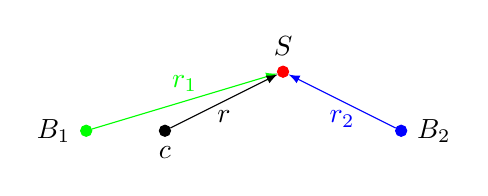
\begin{tikzpicture}[
        point/.style = {circle, draw=#1, fill=#1, node contents={}, inner sep=0.05cm},
        >=latex
        ]

        \node (B1) at (-1,0)     [point=green, label=left:$B_1$];
        \node (B2) at (3,0)      [point=blue, label=right:$B_2$];
        \node (o) at (0,0)      [point=black, label=below:$c$];
        \node (S) at (1.5,0.75)    [point=red, label=above:$S$];

        \draw[->, color=blue] (B2) -> node[below] {$\vv{r}_2$} (S);
        \draw[->, color=green] (B1) -> node[above] {$\vv{r}_1$} (S);
        \draw[->, color=black] (o) -> node[below] {$\vv{r}$} (S);
    \end{tikzpicture}
    \caption{Vectors. Note $d_1$ refers to the distance from $c$ to $B_1$ and $d_2$ refers to the distance from $c$ to $B_2$. Predictably, $d_{12}=d_1+d_2$ is the distance between the bodies}
\end{figure}

Because $\hat{x}$ points from $c$ to $B_2$, which is not inertially stationary, the $xyz$ frame is rotating. Specifically, it is rotating positively about $z$. Because the celestial bodies are in a circular orbit, their rates of rotation about $c$ are constant. This means that the $xyz$ frame rotates at a constant rate of $\vv{\omega}=\Omega\hat{z}$ 

\end{document}
